% !TEX root = ../vr_st.tex

\subsection{Kuratowski embedding and critical radii}\label{sub:filling radii}

\subsubsection{}

Any compact metric space \(\cX\) can be isometrically embedded into the space \(\rL^\infty(\cX)\) of all bounded real-valued functions on \(\cX\) via the map \(x \in \cX \mapsto d_\cX(x,\cdot)\), known as the \defn{Kuratowski embedding}.
The \(\R\)-space obtained by considering radius \(r\) neighborhoods of the image of \(\cX\) is denoted by \(\rU_r(\cX)\).

Throughout the text, Riemannian manifolds are thought of as metric spaces with the geodesic distance.

\subsubsection{}

Following \cite{gromov1983filling}, the \defn{filling radius} of an \(n\)-dimensional closed orientable Riemannian manifold \(\cM\), denoted \(\fillrad(\cM)\), is defined as the infimal \(\epsilon > 0\) such that the fundamental class in \(\rH_n(\cM; \Z)\) vanishes under the inclusion \(\cM \hookrightarrow \rU_\epsilon(\cM)\), where \(\rU_\epsilon(\cM)\) is the \(\epsilon\)-neighborhood of \(\cM\) in \(\rL^\infty(\cX)\).

This definition can be generalized to incorporate different homology coefficients, as explored in \cite{lim2024vietoris}. 
We are interested in working over a field \(\k\), for which we have
\[
\fillrad(\cM; \field) = \min\set[\big]{r \mid (0, r) \in \barc \rH_n(\rU(\cM); \field)}.
\]
This is particularly meaningful when \(\cM\) is connected and not orientable, and \(\k = \Ftwo\).

\subsubsection{}\label{ss:first_critical_value}

Let \(\cM\) be a closed Riemannian manifold.
By \cite[Thm.~3.5]{hausmann1995vietoris} and \cite[Thm.~4.1]{lim2024vietoris}, we know that there exists \(r_\cM > 0\) such that for all \(r \in (0, r_\cM)\) the inclusion \(\cM \to \rU_{r}(\cM)\) is a homotopy equivalence.
This leads to considering the supremum of all such \(r > 0\) for which the inclusion \(\cM \to \rU_r(\cM)\) is a homotopy
equivalence. 
We will refer to this value as the homotopical radius of $\cM$ and denote it by \(\crit(\mathcal{M})\).

\subsubsection{} \label{ss:beta v.s. fillrad}

In \cite[Defn.~9.44]{lim2024vietoris}, the authors define the generalized filling radius of a homology class \(\omega\) in \(X\) as the smallest \(r > 0\) for which \(\omega\) becomes trivial in \(\rU_r(\cX)\), capturing the scale at which \(\omega\) vanishes under the inclusion of \(X\) into its \(r\)-neighborhood.
Below, we consider a weaker version of this concept, which is equivalent to the smallest generalized filling radius among all non-zero homology classes \(\omega\) in \(X\) of a given degree $m$.

Let us fix a field \(\field\) and an integer \(m \in \N\), the \defn{\(m\)-homological radius} of a totally bounded metric space \(\cX\) is defined by
\[
\firstdeath{m}{\cX; \field} =
\min \big\{r \mid (0, r) \in \barc \rH_m(\rU(\cX); \field)\big\},
\]
if \(\rH_m(\cX) \neq 0\).
If \(\rH_m(\cX) = 0\), set \(\firstdeath{m}{\cX} = 0\).
We will omit \(\field\) from the notation when clear from the context.
A more general notion was independently introduced in \cite[Defn.~9.44]{lim2024vietoris}.

Similarly, for a linear cohomology operation \(\theta\), we define the \defn{\(\img_\theta\)-radius} of \(\cX\) by
\[
\firstdeath{\theta}{\cX} = \min \big\{r \mid (0, r) \in \barc \img_\theta(\rU(\cX))\big\},
\]
if \(\img_\theta(\cX) \neq 0\).
If \(\img_\theta(\cX) = 0\), set $\firstdeath{\theta}{\cX} = 0$.
The \(\ker_\theta\)-radius is defined similarly, but we do not use it in this work.

Clearly, if \(\rH_m(\cX) \neq 0\) (resp. \(\img_\theta(\cX) \neq 0\)), then
\[
\crit(\cX) \leq \firstdeath{m}{\cX} \qquad (\text{resp. }\crit(\cX) \leq  \firstdeath{\theta}{\cX}),
\]
and if $\cM$ is connected and $n$-dimensional, then
\[
\firstdeath{n}{\cM} = \fillrad(\cM).
\]


\subsubsection{}\label{ss:kuratowski_vr}

There is a deep relationship between the \(r\)-neighborhood filtration of $\cX$ in $\rL^\infty(\cX)$ and the Vietoris--Rips complex of \(\cX\) at scale \(2r\), stated in the following.

\proposition \cite[Thm.~4.1]{lim2024vietoris} The spaces $\VR_{2r}(\cX)$ and $\rU_r(\cX)$ are naturally homotopy equivalent for every \(r > 0\).

\medskip Due to the natural homotopy equivalence between these filtrations, we will use them interchangeably as needed. 
In particular, this equivalence allows us to bound the Vietoris--Rips barcode of Riemannian pseudomanifolds using their critical radii. 

\subsection{General estimates}\label{ss:barcode_general}

Let \(\cM\) be a closed Riemannian manifold.
Consider \(\ell, m \in \N\) and \(\theta \in \cO(\ell,m)\).
We will simplify notation writing \(R = \diam(\cM),\, \alpha = 2\crit(\cM)\), \(\beta_m = 2\firstdeath{m}{\cM}\), and \(\gamma_\theta = 2\firstdeath{\theta}{\cM}\).
We say a bar $(a, b)$ is \defn{dominated} by another $(c,d)$ if $c \leq a < b \leq d$.

Because $\VR_r(\cM)$ is empty for \(r \leq 0\) and the homotopy type of $\VR_r(\cM)\simeq \rU_{r/2}(\cM)$ remains the homotopy type of $\cM$ for $r \in (0, \alpha)$, bars in \(\barc \rH_m^{\VR}(\cM)\) and $\barc\img_\theta^{\VR}(\cM)$ either start at $0$ or start after $\alpha$.

More precisely, if \(k = \dim \opH_m(\cM) > 0\) then $\barc\rH_m^{\VR}(\cM)$ contains $(0, \beta_m)$ and \((k - 1)\) additional bars of the form \((0, b)\) with \(\beta_m \leq b \leq R\).
Additionally, all other bars are dominated by \((\alpha, R)\).
If \(\dim \opH_m(\cM) = 0\) then all bars in \(\barc\rH_m^{\VR}(\cM)\) are dominated by \((\alpha, R)\).
See the first row of \cref{fig:barcodes_general} for a pictorial representation of these estimates.

A similar analysis applies to $\barc\img_\theta^{\VR}(\cM)$.
See the second row of \cref{fig:barcodes_general} for these estimates.

\begin{figure}
	\centering
	\begin{tikzpicture}[scale=0.52]
	\begin{axis} [
		title = {\LARGE $\barc\opH_m^{\VR}(\cM)$, if $\opH_m(\cM) \neq 0$},
		ticklabel style = {font=\Large},
		axis y line=middle,
		axis x line=middle,
		ytick={0.7,0.95},
		yticklabels={$2\firstdeath{m}{\cM}$,$\diam(\cM)$},
		xtick={0.55,0.95},
		xticklabels={$2\crit(\cM)$, $\diam(\cM)$},
		xmin=-0.015, xmax=1.1,
		ymin=0, ymax=1.1,]
		\addplot [mark=none] coordinates {(0,0) (1,1)};
		\addplot [thick,color=black!20!white,fill=black!30!white,
		fill opacity=0.4]coordinates {
			(0.55,0.95)
			(0.55,0.55)
			(0.95,0.95)
			(0.55,0.95)};
		\addplot [black!40!white,mark=none,dashed, thin] coordinates {(0,0.7) (0.7,0.7)};
		\addplot [black!40!white,mark=none,dashed, thin] coordinates {(0,0.55) (0.55,0.55)};
		\addplot [black!40!white,mark=none,dashed, thin] coordinates {(0.55,0) (0.55,0.55)};
		\addplot[line width=1.5mm, color=black!30!white] coordinates{(0, 0.7) (0, 0.95)};
		\addplot[barccolor,mark=*] (0, 0.7) circle (2pt) node[above right,barccolor]{};
	\end{axis}
\end{tikzpicture}
\begin{tikzpicture}[scale=0.52]
	\begin{axis} [
		title = {\LARGE $\barc\opH_m^{\VR}(\cM)$, if $\opH_m(\cM) = 0$},
		ticklabel style = {font=\Large},
		axis y line=middle,
		axis x line=middle,
		ytick={0.95},
		yticklabels={$\diam(\cM)$},
		xtick={0.55,0.95},
		xticklabels={$2\crit(\cM)$, $\diam(\cM)$},
		xmin=-0.015, xmax=1.1,
		ymin=0, ymax=1.1,]
		\addplot [mark=none] coordinates {(0,0) (1,1)};
		\addplot [thick,color=black!20!white,fill=black!30!white,
		fill opacity=0.4]coordinates {
			(0.55,0.95)
			(0.55,0.55)
			(0.95,0.95)
			(0.55,0.95)};
		\addplot [black!40!white,mark=none,dashed, thin] coordinates {(0,0.55) (0.55,0.55)};
		\addplot [black!40!white,mark=none,dashed, thin] coordinates {(0.55,0) (0.55,0.55)};
	\end{axis}
\end{tikzpicture}

\begin{tikzpicture}[scale=0.52]
	\begin{axis} [
		title={\LARGE $\thetabarc{\cM}$, if $\img\theta_{\cM}\neq 0$},
		ticklabel style = {font=\Large},
		axis y line=middle,
		axis x line=middle,
		ytick={0.7,0.95},
		yticklabels={$2\firstdeath{\theta}{\cM}$,$\diam(\cM)$},
		xtick={0.55,0.95},
		xticklabels={$2\crit(\cM)$, $\diam(\cM)$},
		xmin=-0.015, xmax=1.1,
		ymin=0, ymax=1.1,]
		\addplot [mark=none] coordinates {(0,0) (1,1)};
		\addplot [thick,color=black!20!white,fill=black!30!white,
		fill opacity=0.4]coordinates {
			(0.55,0.95)
			(0.55,0.55)
			(0.95,0.95)
			(0.55,0.95)};
		\addplot [black!40!white,mark=none,dashed, thin] coordinates {(0,0.7) (0.7,0.7)};
		\addplot [black!40!white,mark=none,dashed, thin] coordinates {(0,0.55) (0.55,0.55)};
		\addplot [black!40!white,mark=none,dashed, thin] coordinates {(0.55,0) (0.55,0.55)};
		\addplot[line width=1.5mm, color=black!30!white] coordinates{(0, 0.7) (0, 0.95)};
		\addplot[barccolor,mark=*] (0, 0.7) circle (2pt) node[above right,barccolor]{};
	\end{axis}
\end{tikzpicture}
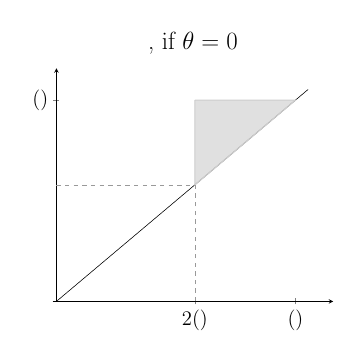
\begin{tikzpicture}[scale=0.52]
	\begin{axis} [
		title={\LARGE $\thetabarc{\cM}$, if $\img\theta_{\cM}= 0$},
		ticklabel style = {font=\Large},
		axis y line=middle,
		axis x line=middle,
		ytick={0.95},
		yticklabels={$\diam(\cM)$},
		xtick={0.55,0.95},
		xticklabels={$2\crit(\cM)$, $\diam(\cM)$},
		xmin=-0.015, xmax=1.1,
		ymin=0, ymax=1.1,]
		\addplot [mark=none] coordinates {(0,0) (1,1)};
		\addplot [thick,color=black!20!white,fill=black!30!white,
		fill opacity=0.4]coordinates {
			(0.55,0.95)
			(0.55,0.55)
			(0.95,0.95)
			(0.55,0.95)};
		\addplot [black!40!white,mark=none,dashed, thin] coordinates {(0,0.55) (0.55,0.55)};
		\addplot [black!40!white,mark=none,dashed, thin] coordinates {(0.55,0) (0.55,0.55)};
	\end{axis}
\end{tikzpicture}
	\caption{Let $\cM$ be a closed Riemannian manifold.
    \emph{Top row:} persistent reduced homology barcodes of $\cM$.
	\emph{Bottom row:} $\img_\theta$-barcodes of $\cM$.
    In each figure, the gray region represents where additional bars could potentially exist within the corresponding barcode.
    See \cref{ss:barcode_general} for details.}
	\label{fig:barcodes_general}
\end{figure}